\documentclass{standalone}
\usepackage{tikz}
\usetikzlibrary{patterns, positioning}


\begin{document}
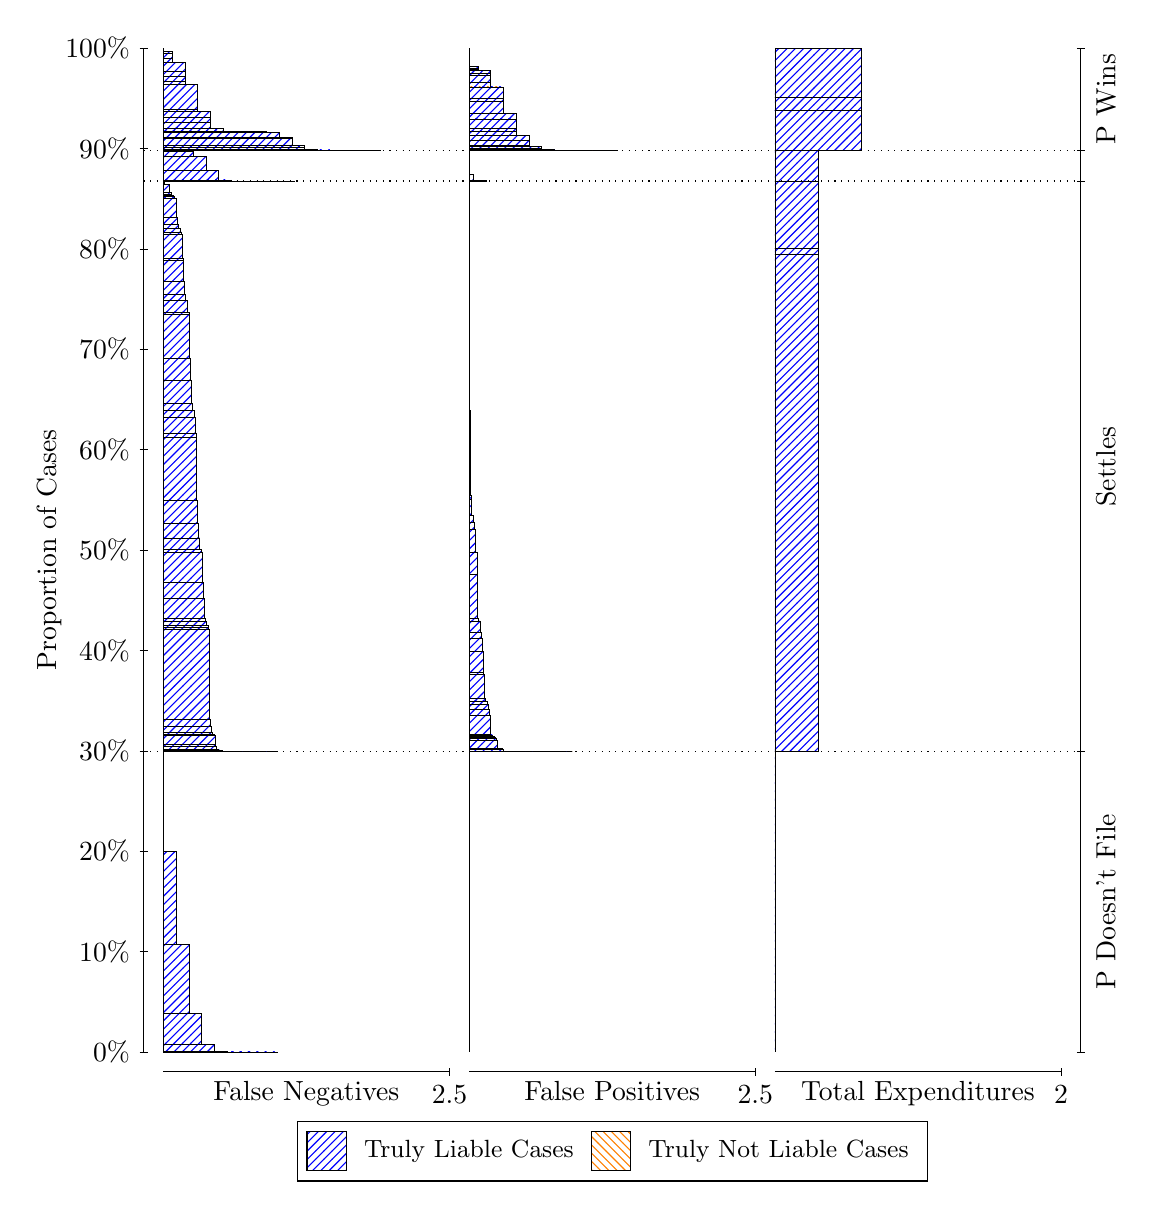
\begin{tikzpicture}
\draw[black, very thin] (1.5,1.75) -- (1.5,14.5);
\node[rotate=90, text=black, anchor=center] at (0.3, 8.125) {Proportion of Cases};
\draw[black, very thin] (1.45,1.75) -- (1.55,1.75);
\node[text=black, anchor=east] at (1.45, 1.75) {0\%};
\draw[black, very thin] (1.45,3.025) -- (1.55,3.025);
\node[text=black, anchor=east] at (1.45, 3.025) {10\%};
\draw[black, very thin] (1.45,4.3) -- (1.55,4.3);
\node[text=black, anchor=east] at (1.45, 4.3) {20\%};
\draw[black, very thin] (1.45,5.575) -- (1.55,5.575);
\node[text=black, anchor=east] at (1.45, 5.575) {30\%};
\draw[black, very thin] (1.45,6.85) -- (1.55,6.85);
\node[text=black, anchor=east] at (1.45, 6.85) {40\%};
\draw[black, very thin] (1.45,8.125) -- (1.55,8.125);
\node[text=black, anchor=east] at (1.45, 8.125) {50\%};
\draw[black, very thin] (1.45,9.4) -- (1.55,9.4);
\node[text=black, anchor=east] at (1.45, 9.4) {60\%};
\draw[black, very thin] (1.45,10.675) -- (1.55,10.675);
\node[text=black, anchor=east] at (1.45, 10.675) {70\%};
\draw[black, very thin] (1.45,11.95) -- (1.55,11.95);
\node[text=black, anchor=east] at (1.45, 11.95) {80\%};
\draw[black, very thin] (1.45,13.225) -- (1.55,13.225);
\node[text=black, anchor=east] at (1.45, 13.225) {90\%};
\draw[black, very thin] (1.45,14.5) -- (1.55,14.5);
\node[text=black, anchor=east] at (1.45, 14.5) {100\%};

\draw[black, very thin] (13.4,1.75) -- (13.4,14.5);
\draw[black, very thin] (13.35,1.75) -- (13.45,1.75);
\node[anchor=west] at (13.35, 1.75) {};
\draw[black, very thin] (13.35,5.563) -- (13.45,5.563);
\node[anchor=west] at (13.35, 5.563) {};
\draw[black, very thin] (13.35,12.811) -- (13.45,12.811);
\node[anchor=west] at (13.35, 12.811) {};
\draw[black, very thin] (13.35,13.204) -- (13.45,13.204);
\node[anchor=west] at (13.35, 13.204) {};
\draw[black, very thin] (13.35,14.5) -- (13.45,14.5);
\node[anchor=west] at (13.35, 14.5) {};

\draw[black, very thin, pattern color=blue, pattern=north east lines] (1.75,1.75) rectangle (3.2033,1.75);
\draw[black, very thin, pattern color=blue, pattern=north east lines] (1.75,1.75) rectangle (3.0419,1.75);
\draw[black, very thin, pattern color=blue, pattern=north east lines] (1.75,1.75) rectangle (2.8804,1.75);
\draw[black, very thin, pattern color=blue, pattern=north east lines] (1.75,1.75) rectangle (2.7189,1.7503);
\draw[black, very thin, pattern color=blue, pattern=north east lines] (1.75,1.7503) rectangle (2.5574,1.7582);
\draw[black, very thin, pattern color=blue, pattern=north east lines] (1.75,1.7582) rectangle (2.3959,1.8434);
\draw[black, very thin, pattern color=blue, pattern=north east lines] (1.75,1.8434) rectangle (2.2344,2.2366);
\draw[black, very thin, pattern color=blue, pattern=north east lines] (1.75,2.2366) rectangle (2.073,3.1157);
\draw[black, very thin, pattern color=blue, pattern=north east lines] (1.75,3.1157) rectangle (1.9115,4.2995);
\draw[black, very thin, pattern color=orange, pattern=north west lines] (1.75,4.2995) rectangle (1.75,4.2995);
\draw[black, very thin, pattern color=blue, pattern=north east lines] (1.75,4.2995) rectangle (1.75,5.563);
\draw[black, very thin, pattern color=blue, pattern=north east lines] (1.75,5.563) rectangle (3.2033,5.563);
\draw[black, very thin, pattern color=blue, pattern=north east lines] (1.75,5.563) rectangle (3.1307,5.563);
\draw[black, very thin, pattern color=blue, pattern=north east lines] (1.75,5.563) rectangle (3.058,5.563);
\draw[black, very thin, pattern color=blue, pattern=north east lines] (1.75,5.563) rectangle (3.0419,5.563);
\draw[black, very thin, pattern color=blue, pattern=north east lines] (1.75,5.563) rectangle (2.9853,5.563);
\draw[black, very thin, pattern color=blue, pattern=north east lines] (1.75,5.563) rectangle (2.9692,5.563);
\draw[black, very thin, pattern color=blue, pattern=north east lines] (1.75,5.563) rectangle (2.9127,5.563);
\draw[black, very thin, pattern color=blue, pattern=north east lines] (1.75,5.563) rectangle (2.8965,5.563);
\draw[black, very thin, pattern color=blue, pattern=north east lines] (1.75,5.563) rectangle (2.8804,5.563);
\draw[black, very thin, pattern color=blue, pattern=north east lines] (1.75,5.563) rectangle (2.84,5.563);
\draw[black, very thin, pattern color=blue, pattern=north east lines] (1.75,5.563) rectangle (2.8239,5.563);
\draw[black, very thin, pattern color=blue, pattern=north east lines] (1.75,5.563) rectangle (2.8077,5.563);
\draw[black, very thin, pattern color=blue, pattern=north east lines] (1.75,5.563) rectangle (2.7673,5.563);
\draw[black, very thin, pattern color=blue, pattern=north east lines] (1.75,5.563) rectangle (2.7512,5.563);
\draw[black, very thin, pattern color=blue, pattern=north east lines] (1.75,5.563) rectangle (2.735,5.563);
\draw[black, very thin, pattern color=blue, pattern=north east lines] (1.75,5.563) rectangle (2.7189,5.563);
\draw[black, very thin, pattern color=blue, pattern=north east lines] (1.75,5.563) rectangle (2.6947,5.563);
\draw[black, very thin, pattern color=blue, pattern=north east lines] (1.75,5.563) rectangle (2.6785,5.5631);
\draw[black, very thin, pattern color=blue, pattern=north east lines] (1.75,5.5631) rectangle (2.6624,5.5631);
\draw[black, very thin, pattern color=blue, pattern=north east lines] (1.75,5.5631) rectangle (2.6462,5.5632);
\draw[black, very thin, pattern color=blue, pattern=north east lines] (1.75,5.5632) rectangle (2.622,5.5636);
\draw[black, very thin, pattern color=blue, pattern=north east lines] (1.75,5.5636) rectangle (2.6059,5.5636);
\draw[black, very thin, pattern color=blue, pattern=north east lines] (1.75,5.5636) rectangle (2.5897,5.5645);
\draw[black, very thin, pattern color=blue, pattern=north east lines] (1.75,5.5645) rectangle (2.5736,5.5652);
\draw[black, very thin, pattern color=blue, pattern=north east lines] (1.75,5.5652) rectangle (2.5574,5.5653);
\draw[black, very thin, pattern color=blue, pattern=north east lines] (1.75,5.5653) rectangle (2.5332,5.5661);
\draw[black, very thin, pattern color=blue, pattern=north east lines] (1.75,5.5661) rectangle (2.517,5.5709);
\draw[black, very thin, pattern color=blue, pattern=north east lines] (1.75,5.5709) rectangle (2.5009,5.5764);
\draw[black, very thin, pattern color=blue, pattern=north east lines] (1.75,5.5764) rectangle (2.4847,5.5778);
\draw[black, very thin, pattern color=blue, pattern=north east lines] (1.75,5.5778) rectangle (2.4767,5.5789);
\draw[black, very thin, pattern color=blue, pattern=north east lines] (1.75,5.5789) rectangle (2.4605,5.5865);
\draw[black, very thin, pattern color=blue, pattern=north east lines] (1.75,5.5865) rectangle (2.4444,5.5885);
\draw[black, very thin, pattern color=blue, pattern=north east lines] (1.75,5.5885) rectangle (2.4282,5.6271);
\draw[black, very thin, pattern color=blue, pattern=north east lines] (1.75,5.6271) rectangle (2.4121,5.6546);
\draw[black, very thin, pattern color=blue, pattern=north east lines] (1.75,5.6546) rectangle (2.404,5.7763);
\draw[black, very thin, pattern color=blue, pattern=north east lines] (1.75,5.7763) rectangle (2.3959,5.7817);
\draw[black, very thin, pattern color=blue, pattern=north east lines] (1.75,5.7817) rectangle (2.3717,5.806);
\draw[black, very thin, pattern color=blue, pattern=north east lines] (1.75,5.806) rectangle (2.3556,5.8814);
\draw[black, very thin, pattern color=blue, pattern=north east lines] (1.75,5.8814) rectangle (2.3394,5.9778);
\draw[black, very thin, pattern color=blue, pattern=north east lines] (1.75,5.9778) rectangle (2.3313,7.1193);
\draw[black, very thin, pattern color=blue, pattern=north east lines] (1.75,7.1193) rectangle (2.3233,7.1415);
\draw[black, very thin, pattern color=blue, pattern=north east lines] (1.75,7.1415) rectangle (2.3152,7.1683);
\draw[black, very thin, pattern color=blue, pattern=north east lines] (1.75,7.1683) rectangle (2.299,7.2219);
\draw[black, very thin, pattern color=blue, pattern=north east lines] (1.75,7.2219) rectangle (2.2829,7.2543);
\draw[black, very thin, pattern color=blue, pattern=north east lines] (1.75,7.2543) rectangle (2.2667,7.5111);
\draw[black, very thin, pattern color=blue, pattern=north east lines] (1.75,7.5111) rectangle (2.2506,7.7165);
\draw[black, very thin, pattern color=blue, pattern=north east lines] (1.75,7.7165) rectangle (2.2425,8.1001);
\draw[black, very thin, pattern color=blue, pattern=north east lines] (1.75,8.1001) rectangle (2.2344,8.1341);
\draw[black, very thin, pattern color=blue, pattern=north east lines] (1.75,8.1341) rectangle (2.2102,8.2777);
\draw[black, very thin, pattern color=blue, pattern=north east lines] (1.75,8.2777) rectangle (2.1941,8.4702);
\draw[black, very thin, pattern color=blue, pattern=north east lines] (1.75,8.4702) rectangle (2.1779,8.7622);
\draw[black, very thin, pattern color=blue, pattern=north east lines] (1.75,8.7622) rectangle (2.1699,9.5546);
\draw[black, very thin, pattern color=blue, pattern=north east lines] (1.75,9.5546) rectangle (2.1618,9.6102);
\draw[black, very thin, pattern color=blue, pattern=north east lines] (1.75,9.6102) rectangle (2.1537,9.8051);
\draw[black, very thin, pattern color=blue, pattern=north east lines] (1.75,9.8051) rectangle (2.1376,9.9002);
\draw[black, very thin, pattern color=blue, pattern=north east lines] (1.75,9.9002) rectangle (2.1214,9.9893);
\draw[black, very thin, pattern color=blue, pattern=north east lines] (1.75,9.9893) rectangle (2.1053,10.278);
\draw[black, very thin, pattern color=blue, pattern=north east lines] (1.75,10.278) rectangle (2.0891,10.562);
\draw[black, very thin, pattern color=blue, pattern=north east lines] (1.75,10.562) rectangle (2.081,11.115);
\draw[black, very thin, pattern color=blue, pattern=north east lines] (1.75,11.115) rectangle (2.073,11.149);
\draw[black, very thin, pattern color=blue, pattern=north east lines] (1.75,11.149) rectangle (2.0487,11.292);
\draw[black, very thin, pattern color=blue, pattern=north east lines] (1.75,11.292) rectangle (2.0326,11.372);
\draw[black, very thin, pattern color=blue, pattern=north east lines] (1.75,11.372) rectangle (2.0164,11.538);
\draw[black, very thin, pattern color=blue, pattern=north east lines] (1.75,11.538) rectangle (2.0084,11.805);
\draw[black, very thin, pattern color=blue, pattern=north east lines] (1.75,11.805) rectangle (2.0003,11.828);
\draw[black, very thin, pattern color=blue, pattern=north east lines] (1.75,11.828) rectangle (1.9922,12.133);
\draw[black, very thin, pattern color=blue, pattern=north east lines] (1.75,12.133) rectangle (1.9761,12.166);
\draw[black, very thin, pattern color=blue, pattern=north east lines] (1.75,12.166) rectangle (1.9599,12.209);
\draw[black, very thin, pattern color=blue, pattern=north east lines] (1.75,12.209) rectangle (1.9438,12.267);
\draw[black, very thin, pattern color=blue, pattern=north east lines] (1.75,12.267) rectangle (1.9276,12.345);
\draw[black, very thin, pattern color=blue, pattern=north east lines] (1.75,12.345) rectangle (1.9196,12.59);
\draw[black, very thin, pattern color=blue, pattern=north east lines] (1.75,12.59) rectangle (1.9115,12.596);
\draw[black, very thin, pattern color=blue, pattern=north east lines] (1.75,12.596) rectangle (1.8873,12.62);
\draw[black, very thin, pattern color=blue, pattern=north east lines] (1.75,12.62) rectangle (1.8711,12.625);
\draw[black, very thin, pattern color=blue, pattern=north east lines] (1.75,12.625) rectangle (1.855,12.644);
\draw[black, very thin, pattern color=blue, pattern=north east lines] (1.75,12.644) rectangle (1.8469,12.67);
\draw[black, very thin, pattern color=blue, pattern=north east lines] (1.75,12.67) rectangle (1.8388,12.671);
\draw[black, very thin, pattern color=blue, pattern=north east lines] (1.75,12.671) rectangle (1.8307,12.765);
\draw[black, very thin, pattern color=blue, pattern=north east lines] (1.75,12.765) rectangle (1.8146,12.767);
\draw[black, very thin, pattern color=blue, pattern=north east lines] (1.75,12.767) rectangle (1.7984,12.77);
\draw[black, very thin, pattern color=blue, pattern=north east lines] (1.75,12.77) rectangle (1.7823,12.773);
\draw[black, very thin, pattern color=blue, pattern=north east lines] (1.75,12.773) rectangle (1.7661,12.777);
\draw[black, very thin, pattern color=blue, pattern=north east lines] (1.75,12.777) rectangle (1.7581,12.803);
\draw[black, very thin, pattern color=orange, pattern=north west lines] (1.75,12.803) rectangle (1.75,12.803);
\draw[black, very thin, pattern color=blue, pattern=north east lines] (1.75,12.803) rectangle (1.75,12.811);
\draw[black, very thin, pattern color=blue, pattern=north east lines] (1.75,12.811) rectangle (3.4213,12.811);
\draw[black, very thin, pattern color=blue, pattern=north east lines] (1.75,12.811) rectangle (3.2599,12.811);
\draw[black, very thin, pattern color=blue, pattern=north east lines] (1.75,12.811) rectangle (3.0984,12.811);
\draw[black, very thin, pattern color=blue, pattern=north east lines] (1.75,12.811) rectangle (2.9369,12.811);
\draw[black, very thin, pattern color=blue, pattern=north east lines] (1.75,12.811) rectangle (2.7754,12.811);
\draw[black, very thin, pattern color=blue, pattern=north east lines] (1.75,12.811) rectangle (2.6139,12.826);
\draw[black, very thin, pattern color=blue, pattern=north east lines] (1.75,12.826) rectangle (2.4524,12.943);
\draw[black, very thin, pattern color=blue, pattern=north east lines] (1.75,12.943) rectangle (2.291,13.122);
\draw[black, very thin, pattern color=blue, pattern=north east lines] (1.75,13.122) rectangle (2.1295,13.193);
\draw[black, very thin, pattern color=blue, pattern=north east lines] (1.75,13.193) rectangle (1.968,13.204);
\draw[black, very thin, pattern color=orange, pattern=north west lines] (1.75,13.204) rectangle (1.75,13.204);
\draw[black, very thin, pattern color=blue, pattern=north east lines] (1.75,13.204) rectangle (4.5113,13.204);
\draw[black, very thin, pattern color=blue, pattern=north east lines] (1.75,13.204) rectangle (4.3499,13.204);
\draw[black, very thin, pattern color=blue, pattern=north east lines] (1.75,13.204) rectangle (4.1884,13.204);
\draw[black, very thin, pattern color=blue, pattern=north east lines] (1.75,13.204) rectangle (4.0269,13.204);
\draw[black, very thin, pattern color=blue, pattern=north east lines] (1.75,13.204) rectangle (4.0269,13.204);
\draw[black, very thin, pattern color=blue, pattern=north east lines] (1.75,13.204) rectangle (3.8654,13.204);
\draw[black, very thin, pattern color=blue, pattern=north east lines] (1.75,13.204) rectangle (3.8654,13.205);
\draw[black, very thin, pattern color=blue, pattern=north east lines] (1.75,13.205) rectangle (3.7039,13.206);
\draw[black, very thin, pattern color=blue, pattern=north east lines] (1.75,13.206) rectangle (3.7039,13.214);
\draw[black, very thin, pattern color=blue, pattern=north east lines] (1.75,13.214) rectangle (3.5424,13.244);
\draw[black, very thin, pattern color=blue, pattern=north east lines] (1.75,13.244) rectangle (3.5424,13.26);
\draw[black, very thin, pattern color=blue, pattern=north east lines] (1.75,13.26) rectangle (3.4779,13.26);
\draw[black, very thin, pattern color=blue, pattern=north east lines] (1.75,13.26) rectangle (3.381,13.349);
\draw[black, very thin, pattern color=blue, pattern=north east lines] (1.75,13.349) rectangle (3.381,13.364);
\draw[black, very thin, pattern color=blue, pattern=north east lines] (1.75,13.364) rectangle (3.3164,13.364);
\draw[black, very thin, pattern color=blue, pattern=north east lines] (1.75,13.364) rectangle (3.2195,13.431);
\draw[black, very thin, pattern color=blue, pattern=north east lines] (1.75,13.431) rectangle (3.1549,13.431);
\draw[black, very thin, pattern color=blue, pattern=north east lines] (1.75,13.431) rectangle (3.1549,13.431);
\draw[black, very thin, pattern color=blue, pattern=north east lines] (1.75,13.431) rectangle (3.058,13.439);
\draw[black, very thin, pattern color=blue, pattern=north east lines] (1.75,13.439) rectangle (2.9934,13.439);
\draw[black, very thin, pattern color=blue, pattern=north east lines] (1.75,13.439) rectangle (2.9934,13.439);
\draw[black, very thin, pattern color=blue, pattern=north east lines] (1.75,13.439) rectangle (2.8965,13.439);
\draw[black, very thin, pattern color=blue, pattern=north east lines] (1.75,13.439) rectangle (2.8965,13.439);
\draw[black, very thin, pattern color=blue, pattern=north east lines] (1.75,13.439) rectangle (2.8319,13.439);
\draw[black, very thin, pattern color=blue, pattern=north east lines] (1.75,13.439) rectangle (2.735,13.439);
\draw[black, very thin, pattern color=blue, pattern=north east lines] (1.75,13.439) rectangle (2.735,13.439);
\draw[black, very thin, pattern color=blue, pattern=north east lines] (1.75,13.439) rectangle (2.735,13.439);
\draw[black, very thin, pattern color=blue, pattern=north east lines] (1.75,13.439) rectangle (2.6704,13.441);
\draw[black, very thin, pattern color=blue, pattern=north east lines] (1.75,13.441) rectangle (2.5736,13.441);
\draw[black, very thin, pattern color=blue, pattern=north east lines] (1.75,13.441) rectangle (2.5736,13.441);
\draw[black, very thin, pattern color=blue, pattern=north east lines] (1.75,13.441) rectangle (2.509,13.448);
\draw[black, very thin, pattern color=blue, pattern=north east lines] (1.75,13.448) rectangle (2.509,13.484);
\draw[black, very thin, pattern color=blue, pattern=north east lines] (1.75,13.484) rectangle (2.4121,13.484);
\draw[black, very thin, pattern color=blue, pattern=north east lines] (1.75,13.484) rectangle (2.4121,13.484);
\draw[black, very thin, pattern color=blue, pattern=north east lines] (1.75,13.484) rectangle (2.3475,13.487);
\draw[black, very thin, pattern color=blue, pattern=north east lines] (1.75,13.487) rectangle (2.3475,13.559);
\draw[black, very thin, pattern color=blue, pattern=north east lines] (1.75,13.559) rectangle (2.3475,13.623);
\draw[black, very thin, pattern color=blue, pattern=north east lines] (1.75,13.623) rectangle (2.3475,13.698);
\draw[black, very thin, pattern color=blue, pattern=north east lines] (1.75,13.698) rectangle (2.2506,13.698);
\draw[black, very thin, pattern color=blue, pattern=north east lines] (1.75,13.698) rectangle (2.186,13.722);
\draw[black, very thin, pattern color=blue, pattern=north east lines] (1.75,13.722) rectangle (2.186,14.038);
\draw[black, very thin, pattern color=blue, pattern=north east lines] (1.75,14.038) rectangle (2.0245,14.076);
\draw[black, very thin, pattern color=blue, pattern=north east lines] (1.75,14.076) rectangle (2.0245,14.142);
\draw[black, very thin, pattern color=blue, pattern=north east lines] (1.75,14.142) rectangle (2.0245,14.206);
\draw[black, very thin, pattern color=blue, pattern=north east lines] (1.75,14.206) rectangle (2.0245,14.315);
\draw[black, very thin, pattern color=blue, pattern=north east lines] (1.75,14.315) rectangle (1.863,14.37);
\draw[black, very thin, pattern color=blue, pattern=north east lines] (1.75,14.37) rectangle (1.863,14.435);
\draw[black, very thin, pattern color=blue, pattern=north east lines] (1.75,14.435) rectangle (1.863,14.453);
\draw[black, very thin, pattern color=orange, pattern=north west lines] (1.75,14.453) rectangle (1.75,14.453);
\draw[black, very thin, pattern color=blue, pattern=north east lines] (1.75,14.453) rectangle (1.75,14.5);
\draw[black, very thin, pattern color=orange, pattern=north west lines] (5.6333,1.75) rectangle (5.6333,1.75);
\draw[black, very thin, pattern color=blue, pattern=north east lines] (5.6333,1.75) rectangle (5.6333,5.563);
\draw[black, very thin, pattern color=orange, pattern=north west lines] (5.6333,5.563) rectangle (6.9413,5.563);
\draw[black, very thin, pattern color=blue, pattern=north east lines] (5.6333,5.563) rectangle (6.9413,5.563);
\draw[black, very thin, pattern color=orange, pattern=north west lines] (5.6333,5.563) rectangle (6.8687,5.563);
\draw[black, very thin, pattern color=blue, pattern=north east lines] (5.6333,5.563) rectangle (6.8687,5.563);
\draw[black, very thin, pattern color=orange, pattern=north west lines] (5.6333,5.563) rectangle (6.796,5.563);
\draw[black, very thin, pattern color=blue, pattern=north east lines] (5.6333,5.563) rectangle (6.796,5.563);
\draw[black, very thin, pattern color=blue, pattern=north east lines] (5.6333,5.563) rectangle (6.7799,5.563);
\draw[black, very thin, pattern color=blue, pattern=north east lines] (5.6333,5.563) rectangle (6.7072,5.563);
\draw[black, very thin, pattern color=orange, pattern=north west lines] (5.6333,5.563) rectangle (6.6507,5.563);
\draw[black, very thin, pattern color=blue, pattern=north east lines] (5.6333,5.563) rectangle (6.6507,5.563);
\draw[black, very thin, pattern color=blue, pattern=north east lines] (5.6333,5.563) rectangle (6.6345,5.563);
\draw[black, very thin, pattern color=blue, pattern=north east lines] (5.6333,5.563) rectangle (6.6184,5.563);
\draw[black, very thin, pattern color=orange, pattern=north west lines] (5.6333,5.563) rectangle (6.578,5.563);
\draw[black, very thin, pattern color=blue, pattern=north east lines] (5.6333,5.563) rectangle (6.578,5.563);
\draw[black, very thin, pattern color=blue, pattern=north east lines] (5.6333,5.563) rectangle (6.5457,5.563);
\draw[black, very thin, pattern color=orange, pattern=north west lines] (5.6333,5.563) rectangle (6.5053,5.563);
\draw[black, very thin, pattern color=blue, pattern=north east lines] (5.6333,5.563) rectangle (6.5053,5.563);
\draw[black, very thin, pattern color=blue, pattern=north east lines] (5.6333,5.563) rectangle (6.4892,5.563);
\draw[black, very thin, pattern color=blue, pattern=north east lines] (5.6333,5.563) rectangle (6.473,5.563);
\draw[black, very thin, pattern color=blue, pattern=north east lines] (5.6333,5.563) rectangle (6.4569,5.563);
\draw[black, very thin, pattern color=orange, pattern=north west lines] (5.6333,5.563) rectangle (6.4327,5.563);
\draw[black, very thin, pattern color=blue, pattern=north east lines] (5.6333,5.563) rectangle (6.4327,5.563);
\draw[black, very thin, pattern color=blue, pattern=north east lines] (5.6333,5.563) rectangle (6.4165,5.563);
\draw[black, very thin, pattern color=blue, pattern=north east lines] (5.6333,5.563) rectangle (6.3842,5.563);
\draw[black, very thin, pattern color=orange, pattern=north west lines] (5.6333,5.563) rectangle (6.36,5.563);
\draw[black, very thin, pattern color=blue, pattern=north east lines] (5.6333,5.563) rectangle (6.36,5.563);
\draw[black, very thin, pattern color=blue, pattern=north east lines] (5.6333,5.563) rectangle (6.3439,5.563);
\draw[black, very thin, pattern color=blue, pattern=north east lines] (5.6333,5.563) rectangle (6.3277,5.563);
\draw[black, very thin, pattern color=blue, pattern=north east lines] (5.6333,5.563) rectangle (6.3116,5.5631);
\draw[black, very thin, pattern color=blue, pattern=north east lines] (5.6333,5.5631) rectangle (6.2954,5.5631);
\draw[black, very thin, pattern color=orange, pattern=north west lines] (5.6333,5.5631) rectangle (6.2873,5.5631);
\draw[black, very thin, pattern color=blue, pattern=north east lines] (5.6333,5.5631) rectangle (6.2873,5.5631);
\draw[black, very thin, pattern color=blue, pattern=north east lines] (5.6333,5.5631) rectangle (6.2712,5.5631);
\draw[black, very thin, pattern color=blue, pattern=north east lines] (5.6333,5.5631) rectangle (6.255,5.5631);
\draw[black, very thin, pattern color=blue, pattern=north east lines] (5.6333,5.5631) rectangle (6.2227,5.5636);
\draw[black, very thin, pattern color=orange, pattern=north west lines] (5.6333,5.5636) rectangle (6.2147,5.5636);
\draw[black, very thin, pattern color=blue, pattern=north east lines] (5.6333,5.5636) rectangle (6.2147,5.5637);
\draw[black, very thin, pattern color=blue, pattern=north east lines] (5.6333,5.5637) rectangle (6.1985,5.5637);
\draw[black, very thin, pattern color=blue, pattern=north east lines] (5.6333,5.5637) rectangle (6.1824,5.5638);
\draw[black, very thin, pattern color=blue, pattern=north east lines] (5.6333,5.5638) rectangle (6.1662,5.5638);
\draw[black, very thin, pattern color=blue, pattern=north east lines] (5.6333,5.5638) rectangle (6.1501,5.5689);
\draw[black, very thin, pattern color=orange, pattern=north west lines] (5.6333,5.5689) rectangle (6.142,5.5689);
\draw[black, very thin, pattern color=blue, pattern=north east lines] (5.6333,5.5689) rectangle (6.142,5.5689);
\draw[black, very thin, pattern color=blue, pattern=north east lines] (5.6333,5.5689) rectangle (6.1339,5.5695);
\draw[black, very thin, pattern color=blue, pattern=north east lines] (5.6333,5.5695) rectangle (6.1259,5.5699);
\draw[black, very thin, pattern color=blue, pattern=north east lines] (5.6333,5.5699) rectangle (6.1097,5.57);
\draw[black, very thin, pattern color=blue, pattern=north east lines] (5.6333,5.57) rectangle (6.0936,5.5706);
\draw[black, very thin, pattern color=orange, pattern=north west lines] (5.6333,5.5706) rectangle (6.0693,5.5706);
\draw[black, very thin, pattern color=blue, pattern=north east lines] (5.6333,5.5706) rectangle (6.0693,5.5709);
\draw[black, very thin, pattern color=blue, pattern=north east lines] (5.6333,5.5709) rectangle (6.0613,5.5966);
\draw[black, very thin, pattern color=blue, pattern=north east lines] (5.6333,5.5966) rectangle (6.0532,5.6011);
\draw[black, very thin, pattern color=blue, pattern=north east lines] (5.6333,5.6011) rectangle (6.037,5.6033);
\draw[black, very thin, pattern color=blue, pattern=north east lines] (5.6333,5.6033) rectangle (6.0209,5.6073);
\draw[black, very thin, pattern color=blue, pattern=north east lines] (5.6333,5.6073) rectangle (6.0047,5.6092);
\draw[black, very thin, pattern color=blue, pattern=north east lines] (5.6333,5.6092) rectangle (5.9886,5.7024);
\draw[black, very thin, pattern color=blue, pattern=north east lines] (5.6333,5.7024) rectangle (5.9805,5.704);
\draw[black, very thin, pattern color=blue, pattern=north east lines] (5.6333,5.704) rectangle (5.9724,5.7301);
\draw[black, very thin, pattern color=blue, pattern=north east lines] (5.6333,5.7301) rectangle (5.9644,5.7487);
\draw[black, very thin, pattern color=blue, pattern=north east lines] (5.6333,5.7487) rectangle (5.9482,5.7543);
\draw[black, very thin, pattern color=blue, pattern=north east lines] (5.6333,5.7543) rectangle (5.9321,5.7773);
\draw[black, very thin, pattern color=blue, pattern=north east lines] (5.6333,5.7773) rectangle (5.9079,5.7835);
\draw[black, very thin, pattern color=blue, pattern=north east lines] (5.6333,5.7835) rectangle (5.8998,6.0292);
\draw[black, very thin, pattern color=blue, pattern=north east lines] (5.6333,6.0292) rectangle (5.8917,6.1067);
\draw[black, very thin, pattern color=blue, pattern=north east lines] (5.6333,6.1067) rectangle (5.8756,6.1649);
\draw[black, very thin, pattern color=blue, pattern=north east lines] (5.6333,6.1649) rectangle (5.8594,6.2082);
\draw[black, very thin, pattern color=blue, pattern=north east lines] (5.6333,6.2082) rectangle (5.8433,6.2408);
\draw[black, very thin, pattern color=blue, pattern=north east lines] (5.6333,6.2408) rectangle (5.8271,6.5459);
\draw[black, very thin, pattern color=blue, pattern=north east lines] (5.6333,6.5459) rectangle (5.819,6.5683);
\draw[black, very thin, pattern color=blue, pattern=north east lines] (5.6333,6.5683) rectangle (5.811,6.8358);
\draw[black, very thin, pattern color=blue, pattern=north east lines] (5.6333,6.8358) rectangle (5.8029,7.0021);
\draw[black, very thin, pattern color=blue, pattern=north east lines] (5.6333,7.0021) rectangle (5.7867,7.0821);
\draw[black, very thin, pattern color=blue, pattern=north east lines] (5.6333,7.0821) rectangle (5.7706,7.2244);
\draw[black, very thin, pattern color=blue, pattern=north east lines] (5.6333,7.2244) rectangle (5.7464,7.2589);
\draw[black, very thin, pattern color=blue, pattern=north east lines] (5.6333,7.2589) rectangle (5.7383,7.8115);
\draw[black, very thin, pattern color=blue, pattern=north east lines] (5.6333,7.8115) rectangle (5.7302,8.0961);
\draw[black, very thin, pattern color=blue, pattern=north east lines] (5.6333,8.0961) rectangle (5.7141,8.3845);
\draw[black, very thin, pattern color=blue, pattern=north east lines] (5.6333,8.3845) rectangle (5.6979,8.4736);
\draw[black, very thin, pattern color=blue, pattern=north east lines] (5.6333,8.4736) rectangle (5.6818,8.5687);
\draw[black, very thin, pattern color=blue, pattern=north east lines] (5.6333,8.5687) rectangle (5.6656,8.7636);
\draw[black, very thin, pattern color=blue, pattern=north east lines] (5.6333,8.7636) rectangle (5.6576,8.8192);
\draw[black, very thin, pattern color=blue, pattern=north east lines] (5.6333,8.8192) rectangle (5.6495,9.6116);
\draw[black, very thin, pattern color=blue, pattern=north east lines] (5.6333,9.6116) rectangle (5.6414,9.9036);
\draw[black, very thin, pattern color=blue, pattern=north east lines] (5.6333,9.9036) rectangle (5.6333,12.811);
\draw[black, very thin, pattern color=orange, pattern=north west lines] (5.6333,12.811) rectangle (5.8513,12.811);
\draw[black, very thin, pattern color=blue, pattern=north east lines] (5.6333,12.811) rectangle (5.8513,12.821);
\draw[black, very thin, pattern color=blue, pattern=north east lines] (5.6333,12.821) rectangle (5.6899,12.892);
\draw[black, very thin, pattern color=blue, pattern=north east lines] (5.6333,12.892) rectangle (5.6333,13.204);
\draw[black, very thin, pattern color=orange, pattern=north west lines] (5.6333,13.204) rectangle (7.5227,13.204);
\draw[black, very thin, pattern color=blue, pattern=north east lines] (5.6333,13.204) rectangle (7.5227,13.204);
\draw[black, very thin, pattern color=orange, pattern=north west lines] (5.6333,13.204) rectangle (7.3612,13.204);
\draw[black, very thin, pattern color=blue, pattern=north east lines] (5.6333,13.204) rectangle (7.3612,13.204);
\draw[black, very thin, pattern color=blue, pattern=north east lines] (5.6333,13.204) rectangle (7.1997,13.204);
\draw[black, very thin, pattern color=orange, pattern=north west lines] (5.6333,13.204) rectangle (7.1997,13.204);
\draw[black, very thin, pattern color=blue, pattern=north east lines] (5.6333,13.204) rectangle (7.1997,13.204);
\draw[black, very thin, pattern color=blue, pattern=north east lines] (5.6333,13.204) rectangle (7.0382,13.204);
\draw[black, very thin, pattern color=blue, pattern=north east lines] (5.6333,13.204) rectangle (7.0382,13.204);
\draw[black, very thin, pattern color=orange, pattern=north west lines] (5.6333,13.204) rectangle (7.0382,13.204);
\draw[black, very thin, pattern color=blue, pattern=north east lines] (5.6333,13.204) rectangle (7.0382,13.204);
\draw[black, very thin, pattern color=orange, pattern=north west lines] (5.6333,13.204) rectangle (6.8767,13.204);
\draw[black, very thin, pattern color=blue, pattern=north east lines] (5.6333,13.204) rectangle (6.8767,13.204);
\draw[black, very thin, pattern color=blue, pattern=north east lines] (5.6333,13.204) rectangle (6.8767,13.204);
\draw[black, very thin, pattern color=blue, pattern=north east lines] (5.6333,13.204) rectangle (6.8767,13.204);
\draw[black, very thin, pattern color=orange, pattern=north west lines] (5.6333,13.204) rectangle (6.7153,13.204);
\draw[black, very thin, pattern color=blue, pattern=north east lines] (5.6333,13.204) rectangle (6.7153,13.21);
\draw[black, very thin, pattern color=blue, pattern=north east lines] (5.6333,13.21) rectangle (6.7153,13.21);
\draw[black, very thin, pattern color=blue, pattern=north east lines] (5.6333,13.21) rectangle (6.5538,13.225);
\draw[black, very thin, pattern color=orange, pattern=north west lines] (5.6333,13.225) rectangle (6.5538,13.225);
\draw[black, very thin, pattern color=blue, pattern=north east lines] (5.6333,13.225) rectangle (6.5538,13.251);
\draw[black, very thin, pattern color=blue, pattern=north east lines] (5.6333,13.251) rectangle (6.3923,13.268);
\draw[black, very thin, pattern color=blue, pattern=north east lines] (5.6333,13.268) rectangle (6.3923,13.33);
\draw[black, very thin, pattern color=orange, pattern=north west lines] (5.6333,13.33) rectangle (6.3923,13.33);
\draw[black, very thin, pattern color=blue, pattern=north east lines] (5.6333,13.33) rectangle (6.3923,13.388);
\draw[black, very thin, pattern color=blue, pattern=north east lines] (5.6333,13.388) rectangle (6.2308,13.448);
\draw[black, very thin, pattern color=blue, pattern=north east lines] (5.6333,13.448) rectangle (6.2308,13.481);
\draw[black, very thin, pattern color=orange, pattern=north west lines] (5.6333,13.481) rectangle (6.2308,13.481);
\draw[black, very thin, pattern color=blue, pattern=north east lines] (5.6333,13.481) rectangle (6.2308,13.599);
\draw[black, very thin, pattern color=blue, pattern=north east lines] (5.6333,13.599) rectangle (6.2308,13.601);
\draw[black, very thin, pattern color=blue, pattern=north east lines] (5.6333,13.601) rectangle (6.2308,13.666);
\draw[black, very thin, pattern color=blue, pattern=north east lines] (5.6333,13.666) rectangle (6.0693,13.819);
\draw[black, very thin, pattern color=blue, pattern=north east lines] (5.6333,13.819) rectangle (6.0693,13.861);
\draw[black, very thin, pattern color=blue, pattern=north east lines] (5.6333,13.861) rectangle (6.0693,14.006);
\draw[black, very thin, pattern color=orange, pattern=north west lines] (5.6333,14.006) rectangle (6.0047,14.006);
\draw[black, very thin, pattern color=blue, pattern=north east lines] (5.6333,14.006) rectangle (6.0047,14.006);
\draw[black, very thin, pattern color=blue, pattern=north east lines] (5.6333,14.006) rectangle (5.9079,14.064);
\draw[black, very thin, pattern color=blue, pattern=north east lines] (5.6333,14.064) rectangle (5.9079,14.155);
\draw[black, very thin, pattern color=blue, pattern=north east lines] (5.6333,14.155) rectangle (5.9079,14.181);
\draw[black, very thin, pattern color=blue, pattern=north east lines] (5.6333,14.181) rectangle (5.9079,14.22);
\draw[black, very thin, pattern color=blue, pattern=north east lines] (5.6333,14.22) rectangle (5.8433,14.22);
\draw[black, very thin, pattern color=orange, pattern=north west lines] (5.6333,14.22) rectangle (5.8433,14.22);
\draw[black, very thin, pattern color=blue, pattern=north east lines] (5.6333,14.22) rectangle (5.8433,14.22);
\draw[black, very thin, pattern color=blue, pattern=north east lines] (5.6333,14.22) rectangle (5.7464,14.236);
\draw[black, very thin, pattern color=blue, pattern=north east lines] (5.6333,14.236) rectangle (5.7464,14.239);
\draw[black, very thin, pattern color=blue, pattern=north east lines] (5.6333,14.239) rectangle (5.7464,14.263);
\draw[black, very thin, pattern color=blue, pattern=north east lines] (5.6333,14.263) rectangle (5.6818,14.263);
\draw[black, very thin, pattern color=orange, pattern=north west lines] (5.6333,14.263) rectangle (5.6818,14.263);
\draw[black, very thin, pattern color=blue, pattern=north east lines] (5.6333,14.263) rectangle (5.6818,14.263);
\draw[black, very thin, pattern color=orange, pattern=north west lines] (5.6333,14.263) rectangle (5.6333,14.263);
\draw[black, very thin, pattern color=blue, pattern=north east lines] (5.6333,14.263) rectangle (5.6333,14.5);
\draw[black, very thin, pattern color=orange, pattern=north west lines] (9.5167,1.75) rectangle (9.5167,1.75);
\draw[black, very thin, pattern color=blue, pattern=north east lines] (9.5167,1.75) rectangle (9.5167,5.563);
\draw[black, very thin, pattern color=orange, pattern=north west lines] (9.5167,5.563) rectangle (10.062,5.563);
\draw[black, very thin, pattern color=blue, pattern=north east lines] (9.5167,5.563) rectangle (10.062,11.877);
\draw[black, very thin, pattern color=orange, pattern=north west lines] (9.5167,11.877) rectangle (10.062,11.877);
\draw[black, very thin, pattern color=blue, pattern=north east lines] (9.5167,11.877) rectangle (10.062,11.957);
\draw[black, very thin, pattern color=orange, pattern=north west lines] (9.5167,11.957) rectangle (10.062,11.957);
\draw[black, very thin, pattern color=blue, pattern=north east lines] (9.5167,11.957) rectangle (10.062,12.811);
\draw[black, very thin, pattern color=orange, pattern=north west lines] (9.5167,12.811) rectangle (10.062,12.811);
\draw[black, very thin, pattern color=blue, pattern=north east lines] (9.5167,12.811) rectangle (10.062,13.204);
\draw[black, very thin, pattern color=orange, pattern=north west lines] (9.5167,13.204) rectangle (10.607,13.204);
\draw[black, very thin, pattern color=blue, pattern=north east lines] (9.5167,13.204) rectangle (10.607,13.71);
\draw[black, very thin, pattern color=orange, pattern=north west lines] (9.5167,13.71) rectangle (10.607,13.71);
\draw[black, very thin, pattern color=blue, pattern=north east lines] (9.5167,13.71) rectangle (10.607,13.869);
\draw[black, very thin, pattern color=orange, pattern=north west lines] (9.5167,13.869) rectangle (10.607,13.869);
\draw[black, very thin, pattern color=blue, pattern=north east lines] (9.5167,13.869) rectangle (10.607,14.5);
\draw[black, dotted] (1.5,5.563) -- (13.4,5.563);
\draw[black, dotted] (1.5,12.811) -- (13.4,12.811);
\draw[black, dotted] (1.5,13.204) -- (13.4,13.204);
\draw[black, very thin] (1.75,1.5) -- (5.3833,1.5);
\node[text=black, anchor=north] at (3.5667, 1.5) {False Negatives};
\draw[black, very thin] (5.3833,1.45) -- (5.3833,1.55);
\node[text=black, anchor=north] at (5.3833, 1.45) {2.5};

\draw[black, very thin] (5.6333,1.5) -- (9.2667,1.5);
\node[text=black, anchor=north] at (7.45, 1.5) {False Positives};
\draw[black, very thin] (9.2667,1.45) -- (9.2667,1.55);
\node[text=black, anchor=north] at (9.2667, 1.45) {2.5};

\draw[black, very thin] (9.5167,1.5) -- (13.15,1.5);
\node[text=black, anchor=north] at (11.333, 1.5) {Total Expenditures};
\draw[black, very thin] (13.15,1.45) -- (13.15,1.55);
\node[text=black, anchor=north] at (13.15, 1.45) {2};

\node[text=black, centered, rotate=90] at (13.72, 3.6565) {P Doesn't File};
\node[text=black, centered, rotate=90] at (13.72, 9.1869) {Settles};

\node[text=black, centered, rotate=90] at (13.72, 13.852) {P Wins};

\draw (7.449999999999999,1.5) node[draw=none] (baseCoordinate) {};
\begin{scope}[align=center]
        \matrix[scale=0.5, draw=black, below=0.5cm of baseCoordinate, nodes={draw}, column sep=0.1cm]{
            \node[rectangle, draw, minimum width=0.5cm, minimum height=0.5cm, pattern color=blue, pattern=north east lines] {}; &
            \node[draw=none, font=\small, text=black] (B) {Truly Liable Cases}; &
            \node[rectangle, draw, minimum width=0.5cm, minimum height=0.5cm, pattern color=orange, pattern=north west lines] {}; &
            \node[draw=none, font=\small, text=black] (B) {Truly Not Liable Cases}; \\
            };
\end{scope}

\end{tikzpicture}
\end{document}